\documentclass[tikz,border=3mm]{standalone}

\usepackage{amsmath, amssymb, extarrows, mathtools}


\usetikzlibrary{matrix,positioning,fit,backgrounds,intersections}
\usetikzlibrary{calc}
\usetikzlibrary{arrows}
\usetikzlibrary{decorations.pathreplacing,calligraphy}



\begin{document}

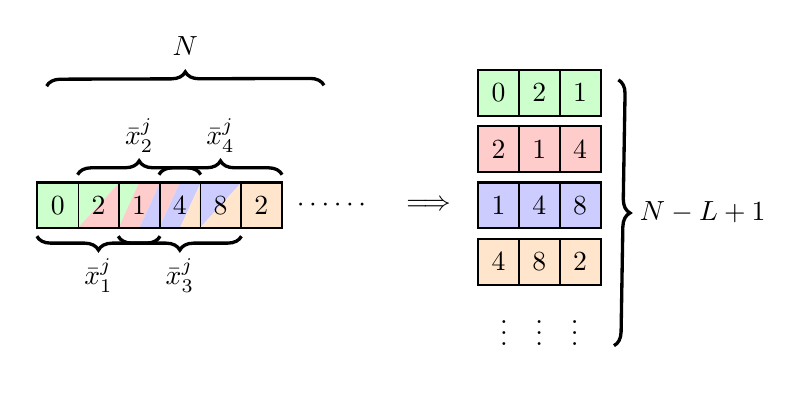
\begin{tikzpicture}[mmat/.style={matrix of math nodes,column sep=-\pgflinewidth/2,
   row sep=-\pgflinewidth/2,cells={nodes={draw,inner sep=5pt,ultra thin}},draw=#1,thick,inner sep=0pt},
   mmat/.default=black,
   node distance=0.3em]
   
   \matrix[mmat](ts_orig){ 0 & 2 & 1 & 4 &8 & 2 \\};
   \node[right=0.05 of ts_orig] (d1) {$\cdots\cdots$};

\node[right=of d1] (split) {$\implies$};

 %timeseries below central one
 \matrix[mmat, right= of split       , name path=ts_split_a0] (ts_split_a0) {1 & 4 & 8 \\ };
 \matrix[mmat, above= of ts_split_a0 , name path=ts_split_a1] (ts_split_a1) {2 & 1 & 4 \\ };
 \matrix[mmat, above= of ts_split_a1 , name path=ts_split_a2] (ts_split_a2) {0 & 2 & 1 \\ };
 \matrix[mmat, below= of ts_split_a0 , name path=ts_split_b0] (ts_split_b0) {4 & 8 & 2 \\ };

 \node[below=of ts_split_b0] (d2) {$\vdots\quad\vdots\quad\vdots$};
 
 \draw [very thick, decorate,decoration={brace,amplitude=5pt,mirror,raise=1mm}]
  (ts_orig-1-1.south west) -- (ts_orig-1-3.south east) node[midway,yshift=-6mm]{$\bar{x}_1^j$};
 \draw [very thick, decorate,decoration={brace,amplitude=5pt,mirror,raise=1mm}]
  (ts_orig-1-3.south west) -- (ts_orig-1-5.south east) node[midway,yshift=-6mm]{$\bar{x}_3^j$};
 \draw [very thick, decorate,decoration={brace,amplitude=5pt,raise=1mm}]
  (ts_orig-1-2.north west) -- (ts_orig-1-4.north east) node[midway,yshift=6mm]{$\bar{x}_2^j$};
 \draw [very thick, decorate,decoration={brace,amplitude=5pt,raise=1mm}]
  (ts_orig-1-4.north west) -- (ts_orig-1-6.north east) node[midway,yshift=6mm]{$\bar{x}_4^j$};

 \node[above=1 of ts_orig-1-1.north west] (b1) {};
 \node[above=1.1 of d1] (b2) {};
 \draw [very thick, decorate,decoration={brace,amplitude=5pt,raise=1mm}]
  (b1) -- (b2) node[midway,yshift=6mm]{$N$};
  
  \node[right=0 of ts_split_a2-1-3.north east] (b3) {};
 \node[right=0.1 of d2.south east] (b4) {};
 \draw [very thick, decorate,decoration={brace,amplitude=5pt,raise=1mm}]
  (b3) -- (b4) node[midway,xshift=12mm]{$N-L+1$};
  
  \begin{scope}[on background layer]
  \fill[green!20  ] (ts_orig-1-1.north west) rectangle (ts_orig-1-1.south east);
  \fill[green!20] (ts_orig-1-2.north east) -- (ts_orig-1-2.north west) --
                  (ts_orig-1-2.south west) -- cycle;
    \fill[red!20] (ts_orig-1-2.south east) -- (ts_orig-1-2.north east) --
                  (ts_orig-1-2.south west) -- cycle;
     \fill[green!20] (ts_orig-1-3.north west) -- (ts_orig-1-3.north) --
                  (ts_orig-1-3.south west) -- cycle;
     \fill[red!20] (ts_orig-1-3.north) -- (ts_orig-1-3.north east) --
                  (ts_orig-1-3.south) -- (ts_orig-1-3.south west) -- cycle;
     \fill[blue!20] (ts_orig-1-3.north east) -- (ts_orig-1-3.south) --
                  (ts_orig-1-3.south east) -- cycle;
    \fill[red!20] (ts_orig-1-4.north west) -- (ts_orig-1-4.north) --
                  (ts_orig-1-4.south west) -- cycle;
     \fill[blue!20] (ts_orig-1-4.north) -- (ts_orig-1-4.north east) --
                  (ts_orig-1-4.south) -- (ts_orig-1-4.south west) -- cycle;
     \fill[orange!20] (ts_orig-1-4.north east) -- (ts_orig-1-4.south) --
                  (ts_orig-1-4.south east) -- cycle;
   \fill[blue!20](ts_orig-1-5.north east) -- (ts_orig-1-5.north west) --
                  (ts_orig-1-5.south west) -- cycle;
    \fill[orange!20] (ts_orig-1-5.south east) -- (ts_orig-1-5.north east) --
                  (ts_orig-1-5.south west) -- cycle;
     \fill[orange!20  ] (ts_orig-1-6.north west) rectangle (ts_orig-1-6.south east);

   \end{scope}  
   
   
    \begin{scope}[on background layer]
  \fill[blue!20  ] (ts_split_a0-1-1.north west) rectangle (ts_split_a0-1-3.south east);
  \fill[red!20   ] (ts_split_a1-1-1.north west) rectangle (ts_split_a1-1-3.south east);
  \fill[green!20 ] (ts_split_a2-1-1.north west) rectangle (ts_split_a2-1-3.south east);
  \fill[orange!20] (ts_split_b0-1-1.north west) rectangle (ts_split_b0-1-3.south east);
   \end{scope}  

  
\end{tikzpicture}

\end{document}